% Practice Test 14 — Texas Edition
% Questions: 30 (21 MC + 9 SA)
% Generated by scripts/generate_practice_tests.py

\begin{practiceQuestion}{1-3-q02}{mc}
\begin{questionText}
In a proportional relationship, the constant of proportionality $k$ equals:
\end{questionText}
\choiceA{$x \div y$}
\choiceB{$y \div x$}
\choiceC{$x \times y$}
\choiceD{$y - x$}
\correctAnswer{B}
\explanation{The constant of proportionality is $k = \frac{y}{x}$, which is the unit rate.}
\end{practiceQuestion}

\begin{practiceQuestion}{1-6-q22}{sa}
\begin{questionText}
Brand A juice: $32$ oz for $\$2.56$. Brand B juice: $48$ oz for $\$3.60$. Which brand has the better price per ounce, and what is it?
\end{questionText}
\correctAnswer{Brand B at $\$0.075$ per oz}
\explanation{A: $2.56 \div 32 = \$0.08$/oz. B: $3.60 \div 48 = \$0.075$/oz. Brand B is cheaper per ounce.}
\end{practiceQuestion}

\begin{practiceQuestion}{2-1-q08}{mc}
\begin{questionText}
$36$ is $45\%$ of what number?
\end{questionText}
\choiceA{$16.2$}
\choiceB{$72$}
\choiceC{$80$}
\choiceD{$90$}
\correctAnswer{C}
\explanation{Divide the part by the percent: $36 \div 0.45 = 80$.}
\end{practiceQuestion}

\begin{practiceQuestion}{2-3-q29}{gsa}
\begin{questionText}
The bar graph shows a store's T-shirt inventory at the start and end of the week. What is the percent decrease?

\begin{center}
\begin{tikzpicture}[scale=0.55]
  \draw[thick,->] (0,0) -- (0,6.5) node[above]{\small T-shirts};
  \draw[thick,->] (0,0) -- (5.5,0);
  % Bars
  \fill[funBlue!60] (0.5,0) rectangle (2,5);
  \fill[funOrange!60] (2.5,0) rectangle (4,3);
  % Labels
  \node[below,font=\small] at (1.25,0) {Start};
  \node[below,font=\small] at (3.25,0) {End};
  \foreach \y/\lab in {1/20,2/40,3/60,4/80,5/100} {
    \draw (-0.1,\y) -- (0.1,\y) node[left,font=\small,xshift=-2pt] {\lab};
  }
  \node[above,font=\small] at (1.25,5) {$100$};
  \node[above,font=\small] at (3.25,3) {$60$};
\end{tikzpicture}
\end{center}
\end{questionText}
\correctAnswer{$40\%$}
\explanation{Change: $100 - 60 = 40$. Percent decrease: $40 \div 100 = 0.40 = 40\%$.}
\end{practiceQuestion}

\begin{practiceQuestion}{2-6-q29}{gsa}
\begin{questionText}
The line graph shows the growth of a $\$1{,}200$ deposit at simple interest. How much interest was earned from Year $0$ to Year $4$?

\begin{center}
\begin{tikzpicture}[scale=0.7]
  \draw[thick,->] (0,0) -- (5.5,0) node[right]{\small Years};
  \draw[thick,->] (0,0) -- (0,5.5) node[above]{\small Total (\$)};
  \draw[gray!20,thin] (0,0) grid[step=1] (5,5);
  \foreach \x in {0,...,4} {
    \node[below,font=\small] at (\x,0) {$\x$};
  }
  \foreach \y/\lab in {1/300,2/600,3/900,4/1200,5/1500} {
    \draw (-0.1,\y) -- (0.1,\y) node[left,font=\small,xshift=-2pt] {\lab};
  }
  % P = 1200, r = 5%, I/year = 60
  % t=0:1200, t=1:1260, t=2:1320, t=3:1380, t=4:1440
  \filldraw[funBlue] (0,4) circle (3pt);
  \filldraw[funBlue] (1,4.2) circle (3pt);
  \filldraw[funBlue] (2,4.4) circle (3pt);
  \filldraw[funBlue] (3,4.6) circle (3pt);
  \filldraw[funBlue] (4,4.8) circle (3pt);
  \draw[thick,funBlue] (0,4) -- (1,4.2) -- (2,4.4) -- (3,4.6) -- (4,4.8);
  \node[above left,font=\small] at (0,4) {$\$1{,}200$};
  \node[above right,font=\small] at (4,4.8) {$\$1{,}440$};
\end{tikzpicture}
\end{center}
\end{questionText}
\correctAnswer{$\$240$}
\explanation{Interest $= 1{,}440 - 1{,}200 = \$240$.}
\end{practiceQuestion}

\begin{practiceQuestion}{2-8-q20}{sa}
\begin{questionText}
Bank A has a $\$4$ monthly fee. Bank B has no monthly fee. How much do you save per year at Bank B?
\end{questionText}
\correctAnswer{$\$48$}
\explanation{$4 \times 12 = \$48$ saved per year.}
\end{practiceQuestion}

\begin{practiceQuestion}{2-9-q22}{sa}
\begin{questionText}
You earn $\$1{,}000$ per month. You save $\$125$. What is your savings rate as a percent?
\end{questionText}
\correctAnswer{$12.5\%$}
\explanation{$\frac{125}{1{,}000} = 0.125 = 12.5\%$.}
\end{practiceQuestion}

\begin{practiceQuestion}{2-10-q24}{sa}
\begin{questionText}
A $\$400$ loan at $12\%$ compounds yearly for $2$ years. How much is owed?
\end{questionText}
\correctAnswer{$\$501.76$}
\explanation{Year 1: $400 \times 1.12 = \$448$. Year 2: $448 \times 1.12 = \$501.76$.}
\end{practiceQuestion}

\begin{practiceQuestion}{4-1-q18}{mc}
\begin{questionText}
Evaluate $\frac{2}{3}a - \frac{1}{2}$ when $a = 6$.


\begin{center}
\fractionCircle{2}{3}
\hspace{1cm}
\fractionCircle{1}{2}
\end{center}
\end{questionText}
\choiceA{$3$}
\choiceB{$3\frac{1}{2}$}
\choiceC{$4$}
\choiceD{$2\frac{1}{2}$}
\correctAnswer{B}
\explanation{Substitute: $\frac{2}{3}(6) - \frac{1}{2} = 4 - \frac{1}{2} = 3\frac{1}{2}$.}
\end{practiceQuestion}

\begin{practiceQuestion}{4-2-q17}{mc}
\begin{questionText}
Simplify $5c + 2d - 3c + 4d$.
\end{questionText}
\choiceA{$8cd$}
\choiceB{$2c + 6d$}
\choiceC{$8c + 6d$}
\choiceD{$2c - 2d$}
\correctAnswer{B}
\explanation{Combine $c$-terms: $5c - 3c = 2c$. Combine $d$-terms: $2d + 4d = 6d$. Result: $2c + 6d$.}
\end{practiceQuestion}

\begin{practiceQuestion}{5-3-q07}{mc}
\begin{questionText}
Solve $3(2x + 1) = 21$.
\end{questionText}
\choiceA{$x = 3$}
\choiceB{$x = 6$}
\choiceC{$x = 10$}
\choiceD{$x = \dfrac{20}{6}$}
\correctAnswer{A}
\explanation{Distribute: $6x + 3 = 21$. Subtract $3$: $6x = 18$. Divide by $6$: $x = 3$. Check: $3(2 \cdot 3 + 1) = 3(7) = 21$ \checkmark.}
\end{practiceQuestion}

\begin{practiceQuestion}{5-4-q06}{mc}
\begin{questionText}
Solve $-0.4y + 2 = 6$.
\end{questionText}
\choiceA{$y = 10$}
\choiceB{$y = -10$}
\choiceC{$y = 20$}
\choiceD{$y = -20$}
\correctAnswer{B}
\explanation{Subtract $2$: $-0.4y = 4$. Divide by $-0.4$: $y = -10$. Check: $-0.4(-10) + 2 = 4 + 2 = 6$ \checkmark.}
\end{practiceQuestion}

\begin{practiceQuestion}{5-5-q28}{gmc}
\begin{questionText}
A store sign shows the rule below. Which inequality represents the sign?

\begin{center}
\begin{tikzpicture}[scale=0.8]
  \draw[thick,rounded corners,fill=funBlue!10] (-0.5,-1.5) rectangle (7,1.5);
  \node[align=center,font=\large] at (3.25,0.4) {\textbf{SALE!}};
  \node[align=center] at (3.25,-0.5) {All items plus $\$5$ tax};
  \node[align=center] at (3.25,-1) {must be \textbf{under} $\$50$};
\end{tikzpicture}
\end{center}

Let $p$ be the price of an item before tax.
\end{questionText}
\choiceA{$p + 5 > 50$}
\choiceB{$p + 5 \leq 50$}
\choiceC{$p + 5 < 50$}
\choiceD{$p + 5 \geq 50$}
\correctAnswer{C}
\explanation{``Under $\$50$'' means strictly less than $50$: $p + 5 < 50$.}
\end{practiceQuestion}

\begin{practiceQuestion}{5-6-q04}{mc}
\begin{questionText}
Solve $3n - 6 > 0$ and describe the graph.
\end{questionText}
\choiceA{Closed circle at $2$, shade right}
\choiceB{Open circle at $2$, shade right}
\choiceC{Open circle at $2$, shade left}
\choiceD{Closed circle at $-2$, shade right}
\correctAnswer{B}
\explanation{Add $6$: $3n > 6$. Divide by $3$: $n > 2$. Open circle at $2$, shade right.}
\end{practiceQuestion}

\begin{practiceQuestion}{6-2-q01}{mc}
\begin{questionText}
A map uses the scale $1$ cm $= 50$ km. You redraw it at $1$ cm $= 25$ km. A road that is $6$ cm on the original map becomes how long on the new map?
\end{questionText}
\choiceA{$3$ cm}
\choiceB{$6$ cm}
\choiceC{$12$ cm}
\choiceD{$150$ cm}
\correctAnswer{C}
\explanation{Scale ratio: $\frac{50}{25} = 2$. New length: $6 \times 2 = 12$ cm. The new scale is more detailed, so the drawing gets bigger.}
\end{practiceQuestion}

\begin{practiceQuestion}{6-3-q03}{mc}
\begin{questionText}
A quadrilateral has four given side lengths: $3$, $4$, $5$, and $6$. How many different quadrilaterals can be drawn?
\end{questionText}
\choiceA{Exactly one}
\choiceB{Exactly two}
\choiceC{More than one}
\choiceD{None — it is impossible}
\correctAnswer{C}
\explanation{Four side lengths alone do not fix the angles of a quadrilateral. Many different shapes are possible with the same four sides.}
\end{practiceQuestion}

\begin{practiceQuestion}{6-4-q17}{mc}
\begin{questionText}
Two angles of a triangle are $25°$ and $25°$. The triangle is:
\end{questionText}
\choiceA{Equilateral}
\choiceB{Isosceles}
\choiceC{Scalene}
\choiceD{Impossible}
\correctAnswer{B}
\explanation{Third angle: $180° - 25° - 25° = 130°$. Two equal angles means two equal sides, making it isosceles.}
\end{practiceQuestion}

\begin{practiceQuestion}{6-5-q26}{gmc}
\begin{questionText}
The diagram shows a rectangular prism being sliced by a horizontal plane (dashed line). What is the cross-section?

\begin{center}
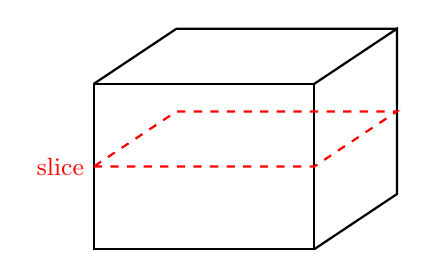
\begin{tikzpicture}[scale=0.7]
  % Rectangular prism
  \draw[thick] (0,0) -- (4,0) -- (4,3) -- (0,3) -- cycle; % front face
  \draw[thick] (4,0) -- (5.5,1) -- (5.5,4) -- (4,3); % right face
  \draw[thick] (0,3) -- (1.5,4) -- (5.5,4); % top face
  \draw[dashed,thick,red] (0,1.5) -- (4,1.5) -- (5.5,2.5) -- (1.5,2.5) -- cycle;
  \node[left,red] at (0,1.5) {\small slice};
\end{tikzpicture}
\end{center}
\end{questionText}
\choiceA{Triangle}
\choiceB{Rectangle}
\choiceC{Circle}
\choiceD{Trapezoid}
\correctAnswer{B}
\explanation{A horizontal slice through a rectangular prism always produces a rectangle congruent to the base.}
\end{practiceQuestion}

\begin{practiceQuestion}{6-8-q12}{mc}
\begin{questionText}
Which method can you use to find a missing side in similar figures?
\end{questionText}
\choiceA{Add the same number to each known side}
\choiceB{Set up a proportion with corresponding sides}
\choiceC{Subtract the scale factor from the known side}
\choiceD{Multiply all sides by the number of vertices}
\correctAnswer{B}
\explanation{In similar figures, corresponding sides are proportional. Set up $\frac{\text{side}_1}{\text{corresponding side}_1} = \frac{\text{side}_2}{\text{corresponding side}_2}$ and cross-multiply.}
\end{practiceQuestion}

\begin{practiceQuestion}{7-4-q20}{sa}
\begin{questionText}
A figure is a rectangle $15$ m by $8$ m with a rectangular hole $5$ m by $3$ m cut out. What is the area of the remaining figure?
\end{questionText}
\correctAnswer{$105$ m$^2$}
\explanation{Outer: $15 \times 8 = 120$ m$^2$. Hole: $5 \times 3 = 15$ m$^2$. Remaining: $120 - 15 = 105$ m$^2$.}
\end{practiceQuestion}

\begin{practiceQuestion}{7-5-q06}{mc}
\begin{questionText}
A gift box is $8$ cm by $5$ cm by $3$ cm. How much wrapping paper is needed to cover the entire box?
\end{questionText}
\choiceA{$79$ cm$^2$}
\choiceB{$120$ cm$^2$}
\choiceC{$158$ cm$^2$}
\choiceD{$316$ cm$^2$}
\correctAnswer{C}
\explanation{$SA = 2(8 \times 5) + 2(8 \times 3) + 2(5 \times 3) = 80 + 48 + 30 = 158$ cm$^2$.}
\end{practiceQuestion}

\begin{practiceQuestion}{7-6-q22}{sa}
\begin{questionText}
A rectangular aquarium is $80$ cm long, $40$ cm wide, and $50$ cm tall. What is its volume in cubic centimeters?
\end{questionText}
\correctAnswer{$160{,}000$ cm$^3$}
\explanation{$V = 80 \times 40 \times 50 = 160{,}000$ cm$^3$.}
\end{practiceQuestion}

\begin{practiceQuestion}{8-1-q28}{gmc}
\begin{questionText}
The table below shows the results of two samples taken from a population of $1{,}000$ students.

\begin{center}
\begin{tabular}{|l|c|c|}
\hline
 & \textbf{Sample 1 (50 students)} & \textbf{Sample 2 (50 students)} \\
\hline
Prefer Math & $18$ & $22$ \\
\hline
Prefer Science & $14$ & $12$ \\
\hline
Prefer English & $10$ & $8$ \\
\hline
Prefer Art & $8$ & $8$ \\
\hline
\end{tabular}
\end{center}

Based on both samples, the best prediction for how many of the $1{,}000$ students prefer math is:
\end{questionText}
\choiceA{$180$}
\choiceB{$220$}
\choiceC{$400$}
\choiceD{$360$}
\correctAnswer{C}
\explanation{Average the two samples: $\frac{18+22}{2} = 20$ out of $50 = 40\%$. Then $40\%$ of $1{,}000 = 400$.}
\end{practiceQuestion}

\begin{practiceQuestion}{8-2-q06}{mc}
\begin{questionText}
A random sample of $30$ trees in a forest has a mean height of $45$ feet. Another random sample of $30$ trees has a mean height of $48$ feet. What is the best estimate for the population mean?
\end{questionText}
\choiceA{$45$ feet}
\choiceB{$48$ feet}
\choiceC{$46.5$ feet}
\choiceD{$93$ feet}
\correctAnswer{C}
\explanation{Average the two sample means: $\frac{45+48}{2} = 46.5$ feet.}
\end{practiceQuestion}

\begin{practiceQuestion}{8-4-q25}{sa}
\begin{questionText}
Team A: mean $88$, range $12$, MAD $3$. Team B: mean $84$, range $30$, MAD $8$. Which team is stronger overall? Justify your answer using at least two measures.
\end{questionText}
\correctAnswer{Team A — higher mean ($88$ vs.\ $84$) and more consistent (MAD $3$ vs.\ $8$, range $12$ vs.\ $30$)}
\explanation{Team A has a higher center (mean $88$) and less variability (smaller MAD and range), meaning Team A is both better on average and more consistent.}
\end{practiceQuestion}

\begin{practiceQuestion}{8-5-q27}{gmc}
\begin{questionText}
The back-to-back stem-and-leaf plot compares quiz scores for two classes.

\begin{center}
\begin{tabular}{r|c|l}
\textbf{Class A} & \textbf{Stem} & \textbf{Class B} \\
\hline
$5\;\;2$ & $6$ & $3\;\;5\;\;8$ \\
$8\;\;5\;\;3\;\;0$ & $7$ & $2\;\;4\;\;9$ \\
$6\;\;4$ & $8$ & $1\;\;3\;\;5\;\;7$ \\
$2$ & $9$ & $0\;\;5$
\end{tabular}

Key: $5 \mid 7$ means $75$ (Class A) and $7 \mid 2$ means $72$ (Class B)
\end{center}

Which class has a higher median?
\end{questionText}
\choiceA{Class A}
\choiceB{Class B}
\choiceC{They have the same median}
\choiceD{Cannot be determined}
\correctAnswer{B}
\explanation{Class A data ($9$ values): $62, 65, 70, 73, 75, 78, 84, 86, 92$. Median $= 75$. Class B data ($12$ values): $63, 65, 68, 72, 74, 79, 81, 83, 85, 87, 90, 95$. Median $= \frac{79+81}{2} = 80$. Class B has a higher median.}
\end{practiceQuestion}

\begin{practiceQuestion}{8-6-q09}{mc}
\begin{questionText}
In a circle graph, two sectors have angles of $144°$ and $72°$. Together, what percent of the whole do they represent?
\end{questionText}
\choiceA{$50\%$}
\choiceB{$60\%$}
\choiceC{$72\%$}
\choiceD{$80\%$}
\correctAnswer{B}
\explanation{$\frac{144 + 72}{360} = \frac{216}{360} = 0.60 = 60\%$.}
\end{practiceQuestion}

\begin{practiceQuestion}{9-4-q16}{mc}
\begin{questionText}
A game has $4$ outcomes: Win Big, Win Small, Lose Small, Lose Big. The probabilities are $0.05$, $0.25$, $0.45$, and $0.25$. Which outcome is LEAST likely?
\end{questionText}
\choiceA{Win Big}
\choiceB{Win Small}
\choiceC{Lose Small}
\choiceD{Lose Big}
\correctAnswer{A}
\explanation{Win Big has the smallest probability ($0.05$), making it least likely.}
\end{practiceQuestion}

\begin{practiceQuestion}{9-6-q11}{mc}
\begin{questionText}
Two dice are rolled. What is the probability that the sum is even?
\end{questionText}
\choiceA{$\frac{1}{4}$}
\choiceB{$\frac{1}{3}$}
\choiceC{$\frac{1}{2}$}
\choiceD{$\frac{2}{3}$}
\correctAnswer{C}
\explanation{Even sums occur when both dice are even or both are odd. Both even: $3 \times 3 = 9$. Both odd: $3 \times 3 = 9$. Total: $18$ out of $36$. $P = \frac{18}{36} = \frac{1}{2}$.}
\end{practiceQuestion}

\begin{practiceQuestion}{9-7-q03}{mc}
\begin{questionText}
To simulate an event with a $\frac{1}{6}$ probability, which tool would be most appropriate?
\end{questionText}
\choiceA{A coin}
\choiceB{A standard die}
\choiceC{A spinner with $4$ sections}
\choiceD{A bag with $2$ marbles}
\correctAnswer{B}
\explanation{A standard die has $6$ equally likely outcomes, each with probability $\frac{1}{6}$.}
\end{practiceQuestion}
